\section{\RU{И если много}\EN{A lot of cases}}

\RU{Если ветвлений слишком много, то генерировать слишком длинный код с многочисленными \JE/\JNE 
уже не так удобно.}
\EN{If a \TT{switch()} statement contains a lot of cases, it is not very convenient for the compiler to emit too large code
with a lot \JE/\JNE instructions.}

\lstinputlisting[label=switch_lot_c]{patterns/08_switch/2_lot/lot.c}

\subsection{x86}

\subsubsection{\NonOptimizing MSVC}

\RU{Рассмотрим пример, скомпилированный в}\EN{We get} (MSVC 2010):

\lstinputlisting[caption=MSVC 2010]{patterns/08_switch/2_lot/lot_msvc.asm.\LANG}

\index{jumptable}
\RU{Здесь происходит следующее: в теле функции есть набор вызовов \printf с разными аргументами. 
Все они имеют, конечно же, адреса, а также внутренние символические метки, которые присвоил им компилятор.
Также все эти метки указываются во внутренней таблице \TT{\$LN11@f}.}
\EN{What we see here is a set of \printf calls with various arguments. 
All they have not only addresses in the memory of the process, but also internal symbolic labels assigned 
by the compiler. 
All these labels are also mentioned in the \TT{\$LN11@f} internal table.}

\RU{В начале функции, если $a$ больше 4, то сразу происходит переход на метку \TT{\$LN1@f}, 
где вызывается \printf с аргументом \TT{'something unknown'}.}
\EN{At the function start, if $a$ is greater than 4, control flow is passed to label 
\TT{\$LN1@f}, where \printf with argument \TT{'something unknown'} is called.}

\RU{А если $a$ меньше или равно 4, то это значение умножается на 4 и прибавляется адрес таблицы 
с переходами (\TT{\$LN11@f}). 
Таким образом, получается адрес внутри таблицы, где лежит нужный адрес внутри тела функции. 
Например, возьмем $a$ равным 2. $2*4 = 8$ (ведь все элементы таблицы~--- это адреса внутри 32-битного процесса, 
таким образом, каждый элемент занимает 4 байта). 8 прибавить к \TT{\$LN11@f}~--- это будет элемент таблицы,
где лежит \TT{\$LN4@f}. \JMP вытаскивает из таблицы адрес \TT{\$LN4@f} и делает безусловный переход туда.}
\EN{But if the value of $a$ is less or equals to 4, then it gets multiplied by 4 and added with the \TT{\$LN11@f} 
table address. That is how an address inside the table is constructed, pointing exactly to the 
element we need. For example, let's say $a$ is equal to 2. $2*4 = 8$ (all table elements 
are addresses in a 32-bit process and that is why all elements are 4 bytes wide). 
The address of the \TT{\$LN11@f} table + 8 is the table element where the \TT{\$LN4@f} label is stored.
\JMP fetches the \TT{\$LN4@f} address from the table and jumps to it.}

\RU{Эта таблица иногда называется}\EN{This table is sometimes called} \IT{jumptable} \OrENRU 
\IT{branch table}\footnote{\EN{The whole method was once called}\RU{Сам метод раньше назывался} 
\IT{computed GOTO} \EN{in early versions of FORTRAN}\RU{В ранних версиях FORTRAN}:
\href{http://go.yurichev.com/17122}{wikipedia}.
\EN{Not quite relevant these days, but what a term}\RU{Не очень-то и полезно в наше время, но
каков термин}!}.

\RU{А там вызывается \printf с аргументом \TT{'two'}. 
Дословно, инструкция \TT{jmp DWORD PTR \$LN11@f[ecx*4]} 
означает \IT{перейти по DWORD, который лежит по адресу} \TT{\$LN11@f + ecx * 4}.}
\EN{Then the corresponding \printf is called with argument \TT{'two'}. 
Literally, the \TT{jmp DWORD PTR \$LN11@f[ecx*4]} instruction implies
\IT{jump to the DWORD that is stored at address} \TT{\$LN11@f + ecx * 4}.}

\ifx\LITE\undefined
\TT{npad} 
(\myref{sec:npad})
\fi
\RU{это макрос ассемблера, выравнивающий начало таблицы, 
чтобы она располагалась по адресу кратному 4 (или 16).
Это нужно для того, чтобы процессор мог эффективнее загружать 32-битные 
значения из памяти через шину с памятью, кэш-память, \etc.}
\EN{is assembly language macro that aligning the next label so that it is to be stored at an address aligned on a 4 byte
(or 16 byte) boundary.
This is very suitable for the processor since it is able to fetch 32-bit values from memory through the memory bus,
cache memory, etc, in a more effective way if it is aligned.}

\ifdefined\IncludeOlly
\clearpage
\myparagraph{\olly}
\index{\olly}

\RU{Попробуем этот пример в}\EN{Let's try this example in} \olly.
\RU{Входное значение функции}\EN{The input value of the function} (2) \RU{загружается в}\EN{is loaded into} \EAX: 

\begin{figure}[H]
\centering
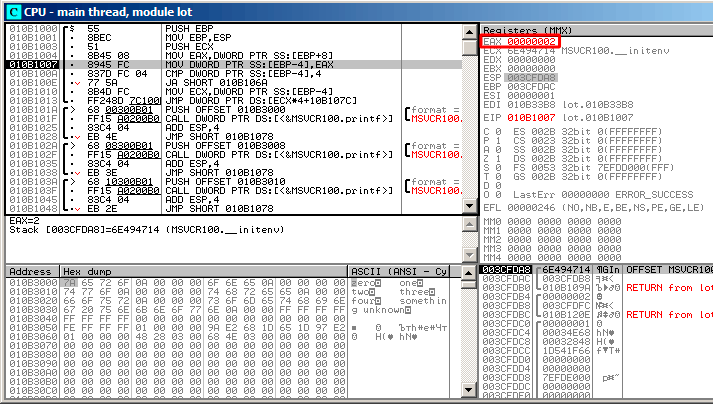
\includegraphics[scale=\FigScale]{patterns/08_switch/2_lot/olly1.png}
\caption{\olly: \RU{входное значение функции загружено в}\EN{function's input value is loaded in} \EAX}
\label{fig:switch_lot_olly1}
\end{figure}

\clearpage
\RU{Входное значение проверяется, не больше ли оно чем}\EN{The input value is checked, is it bigger than} 4? 
\RU{Нет, переход по умолчанию (\q{default}) не будет исполнен}\EN{If not, the \q{default} jump is not 
taken}:
\begin{figure}[H]
\centering
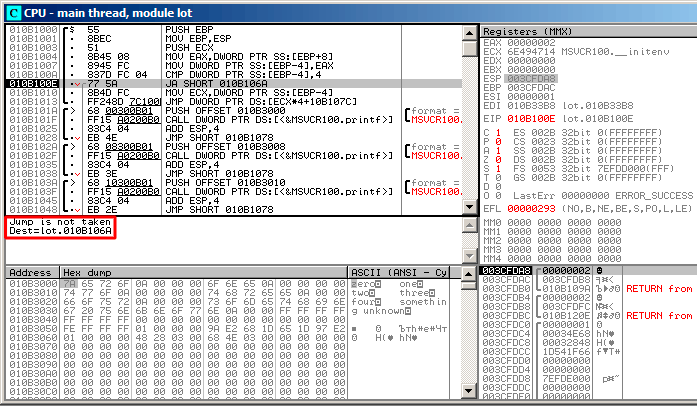
\includegraphics[scale=\FigScale]{patterns/08_switch/2_lot/olly2.png}
\caption{\olly: 2 \RU{не больше чем}\EN{is no bigger than} 4: \RU{переход не сработает}\EN{no jump is taken}}
\label{fig:switch_lot_olly2}
\end{figure}

\clearpage
\RU{Здесь мы видим}\EN{Here we see a} jumptable:

\begin{figure}[H]
\centering
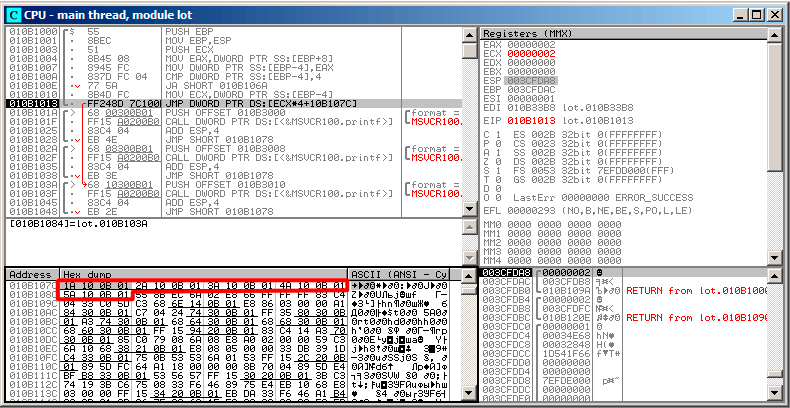
\includegraphics[scale=\FigScale]{patterns/08_switch/2_lot/olly3.png}
\caption{\olly: \RU{вычисляем адрес для перехода используя}\EN{calculating destination address using} jumptable}
\label{fig:switch_lot_olly3}
\end{figure}

\RU{Кстати, щелкнем по \q{Follow in Dump} $\rightarrow$ \q{Address constant}, так что теперь \IT{jumptable} видна в окне данных.}%
\EN{Here we've clicked \q{Follow in Dump} $\rightarrow$ \q{Address constant}, so now we see the \IT{jumptable} in the data window.}
\RU{Это 5 32-битных значений}\EN{These are 5 32-bit values}\footnote{\EN{They are underlined by \olly because
these are also FIXUPs}\RU{Они подчеркнуты в \olly, потому что это также и FIXUP-ы}: \myref{subsec:relocs}, 
\RU{мы вернемся к ним позже}\EN{we are going to come back to them later}}.
\ECX \RU{сейчас содержит}\EN{is now} 2\RU{, так что второй элемент (считая с нулевого) таблицы
будет использован}\EN{, so the second element (counting from zero) of the table is to be used}.
\RU{Кстати, можно также щелкнуть}\EN{It's also possible to click} \q{Follow in Dump} $\rightarrow$ 
\q{Memory address} \AndENRU \olly 
\RU{покажет элемент, который сейчас адресуется в инструкции \JMP}%
\EN{will show the element addressed by the \JMP instruction}. 
\RU{Это}\EN{That's} \TT{0x010B103A}.

\clearpage
\RU{Переход сработал и мы теперь на}\EN{After the jump we are at} \TT{0x010B103A}: 
\RU{сейчас будет исполнен код, выводящий строку}\EN{the code printing} \q{two}\EN{ will now be executed}:

\begin{figure}[H]
\centering
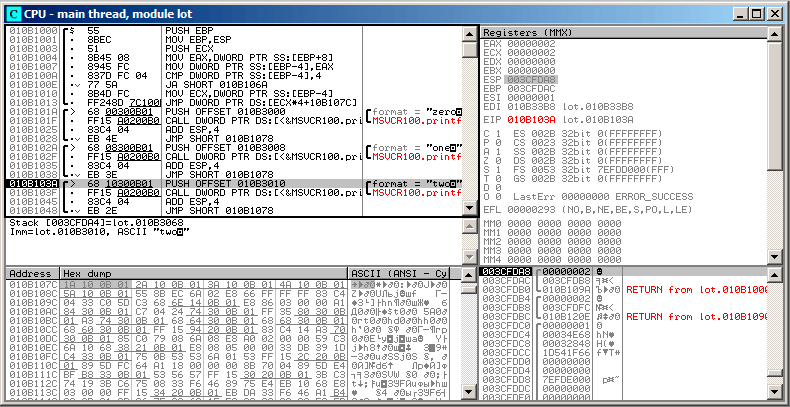
\includegraphics[scale=\FigScale]{patterns/08_switch/2_lot/olly4.png}
\caption{\olly: \RU{теперь мы на соответствующей метке}\EN{now we at the} \IT{case:}\EN{ label}}
\label{fig:switch_lot_olly4}
\end{figure}

\fi

\subsubsection{\NonOptimizing GCC}
\label{switch_lot_GCC}

\RU{Посмотрим, что сгенерирует GCC 4.4.1}\EN{Let's see what GCC 4.4.1 generates}:

\lstinputlisting[caption=GCC 4.4.1]{patterns/08_switch/2_lot/lot_gcc.asm}

\index{x86!\Registers!JMP}
\RU{Практически то же самое, за исключением мелкого нюанса: аргумент из \TT{arg\_0} умножается на 4 
при помощи сдвига влево на 2 бита (это почти то же самое что и умножение на 4)~(\myref{SHR}).
Затем адрес метки внутри функции берется из массива \TT{off\_804855C} и адресуется при помощи 
вычисленного индекса.}
\EN{It is almost the same, with a little nuance: argument \TT{arg\_0} is multiplied by 4 by
shifting it to left by 2 bits (it is almost the same as multiplication by 4)~(\myref{SHR}).
Then the address of the label is taken from the \TT{off\_804855C} array, stored in 
\EAX, and then \TT{JMP EAX} does the actual jump.}


\ifdefined\IncludeARM
\subsection{ARM: \OptimizingKeilVI (\ARMMode)}
\label{sec:SwitchARMLot}

\lstinputlisting[caption=\OptimizingKeilVI (\ARMMode)]{patterns/08_switch/2_lot/lot_ARM_ARM_O3.asm}

\RU{В этом коде используется та особенность режима ARM, 
что все инструкции в этом режиме имеют фиксированную длину 4 байта.}
\EN{This code makes use of the ARM mode feature in which all instructions have a fixed size of 4 bytes.}

\RU{Итак, не будем забывать, что максимальное значение для $a$ это 4: всё что выше, должно вызвать
вывод строки \IT{<<something unknown\textbackslash{}n>>}.}
\EN{Let's keep in mind that the maximum value for $a$ is 4 and any greater value will cause
\IT{<<something unknown\textbackslash{}n>>} string to be printed.}

\index{ARM!\Instructions!CMP}
\index{ARM!\Instructions!ADDCC}
\RU{Самая первая инструкция}\EN{The first} \TT{CMP R0, \#5} 
\RU{сравнивает входное значение в $a$ c 5.}
\EN{instruction compares the input value of $a$ with 5.}

\RU{Следующая инструкция}\EN{The next} \TT{ADDCC PC, PC, R0,LSL\#2}
\footnote{ADD\EMDASH\RU{складывание чисел}\EN{addition}}
\RU{сработает только в случае если}\EN{instruction is being executed only if} $R0 < 5$ (\IT{CC=Carry clear / Less than}). 
\RU{Следовательно, если}\EN{Consequently, if} \TT{ADDCC} \RU{не сработает}\EN{does not trigger} 
(\RU{это случай с}\EN{it is a} $R0 \geq 5$\EN{ case}), 
\RU{выполнится переход на метку}\EN{a jump to} 
\IT{default\_case}\EN{ label will occur}.

\RU{Но если}\EN{But if} $R0 < 5$ \AndENRU \TT{ADDCC} \RU{сработает, то произойдет следующее.}
\EN{triggers, the following is to be happen:}

\RU{Значение в \Reg{0} умножается на 4}\EN{The value in \Reg{0} is multiplied by 4}.
\RU{Фактически}\EN{In fact}, \TT{LSL\#2} \RU{в суффиксе инструкции означает \q{сдвиг влево на 2 бита}.}
\EN{at the instruction's suffix stands for \q{shift left by 2 bits}.}
\RU{Но как будет видно позже}\EN{But as we will see later}~(\myref{division_by_shifting}) \RU{в секции}\EN{in section} 
\q{\ShiftsSectionName}, 
\RU{сдвиг влево на 2 бита эквивалентeн его умножению на 4.}
\EN{shift left by 2 bits is equivalent to multiplying by 4.}

\RU{Затем полученное}\EN{Then we add} $R0*4$ \RU{прибавляется к текущему значению \ac{PC}}\EN{to
the current value in \ac{PC}}, 
\RU{совершая, таким образом, переход на одну из расположенных ниже инструкций \TT{B} (\IT{Branch}).}
\EN{thus jumping to one of the \TT{B} (\IT{Branch}) instructions located below.}

\RU{На момент исполнения}\EN{At the moment of the execution of} \TT{ADDCC},
\RU{содержимое \ac{PC} на 8 байт больше}\EN{the value in \ac{PC} is 8 bytes ahead} (\TT{0x180})%
\RU{, чем адрес по которому расположена сама инструкция} 
\EN{than the address at which the} \TT{ADDCC}\EN{ instruction is located} (\TT{0x178}), 
\RU{либо, говоря иным языком, на 2 инструкции больше.}
\EN{or, in other words, 2 instructions ahead.}

\index{ARM!\RU{Конвейер}\EN{Pipeline}}
\RU{Это связано с работой конвейера процессора ARM:
пока исполняется инструкция \TT{ADDCC}, процессор уже начинает обрабатывать инструкцию после следующей, 
поэтому \ac{PC} указывает туда. Этот факт нужно запомнить.}
\EN{This is how the pipeline in ARM processors works: when \TT{ADDCC} is executed,
the processor at the moment
is beginning to process the instruction after the next one,
so that is why \ac{PC} points there. This has to be memorized.}

\RU{Если $a=0$, тогда к \ac{PC} ничего не будет прибавлено и 
в \ac{PC} запишется актуальный на тот момент \ac{PC} (который больше на 8) 
и произойдет переход на метку \IT{loc\_180}. 
Это на 8 байт дальше места, где находится инструкция \TT{ADDCC}.}
\EN{If $a=0$, then is to be added to the value in \ac{PC},
and the actual value of the \ac{PC} will be written into \ac{PC} (which is 8 bytes ahead)
and a jump to the label \IT{loc\_180} will happen,
which is 8 bytes ahead of the point where the \TT{ADDCC} instruction is.}

\RU{Если}\EN{If} $a=1$, \RU{тогда в \ac{PC} запишется}\EN{then} 
$PC+8+a*4 = PC+8+1*4 = PC+12 = 0x184$\RU{. Это адрес метки \IT{loc\_184}}\EN{ will be written to \ac{PC},
which is the address of the \IT{loc\_184} label}.

\RU{При каждой добавленной к $a$ единице итоговый \ac{PC} увеличивается на 4.}
\EN{With every 1 added to $a$, the resulting \ac{PC} is increased by 4.}
\RU{4 это длина инструкции в режиме ARM и одновременно с этим, 
длина каждой инструкции \TT{B}, их здесь следует 5 в ряд.}
\EN{4 is the instruction length in ARM mode and also, the length of each \TT{B} instruction,
of which there are 5 in row.}

\RU{Каждая из этих пяти инструкций \TT{B} передает управление дальше, где собственно и происходит то, 
что запрограммировано в операторе}
\EN{Each of these five \TT{B} instructions passes control further, to 
what was programmed in the}
\IT{switch()}.
\RU{Там происходит загрузка указателя на свою строку,}
\EN{Pointer loading of the corresponding string occurs there,}\etc{}.

\subsection{ARM: \OptimizingKeilVI (\ThumbMode)}

\lstinputlisting[caption=\OptimizingKeilVI (\ThumbMode)]{patterns/08_switch/2_lot/lot_ARM_thumb_O3.asm}

\index{ARM!\ThumbMode}
\index{ARM!\ThumbTwoMode}
\RU{В режимах Thumb и Thumb-2 уже нельзя надеяться на то, что все инструкции имеют одну длину.}
\EN{One cannot be sure that all instructions in Thumb and Thumb-2 modes has the same size.}
\RU{Можно даже сказать, что в этих режимах инструкции переменной длины, как в x86.}
\EN{It can even be said that in these modes the instructions have variable lengths, just like in x86.}

\index{jumptable}
\RU{Так что здесь добавляется специальная таблица, содержащая информацию о том, как много вариантов здесь,
не включая варианта по умолчанию, и смещения, для каждого варианта. Каждое смещение кодирует метку, куда нужно передать
управление в соответствующем случае.}
\EN{So there is a special table added that contains information about how much cases are there (not including 
default-case), and an offset for each with a label to which control must be passed in 
the corresponding case.}

\index{ARM!\RU{Переключение режимов}\EN{Mode switching}}
\index{ARM!\Instructions!BX}
\RU{Для того чтобы работать с таблицей и совершить переход, вызывается служебная функция}
\EN{A special function is present here in order to deal with the table and pass control, named}
\IT{\_\_ARM\_common\_switch8\_thumb}. 
\RU{Она начинается с инструкции}\EN{It starts with} \TT{BX PC}
\RU{, чья функция~--- переключить процессор в ARM-режим.}
\EN{, whose function is to switch the processor to ARM-mode.}
\RU{Далее функция, работающая с таблицей.}\EN{Then you see the function for table processing.} 
\RU{Она слишком сложная для рассмотрения в данном месте, так что пропустим это.}
\EN{It is too complex to describe it here now, so let's omit it.}
% TODO explain it...

\index{ARM!\Registers!Link Register}
\RU{Но можно отметить, что эта функция использует регистр \ac{LR} как указатель на таблицу.}
\EN{It is interesting to note that the function uses the \ac{LR} register as a pointer to the table.}
\RU{Действительно, после вызова этой функции, 
в \ac{LR} был записан адрес после инструкции}
\EN{Indeed, after calling of this function, \ac{LR} contains the address after}
\TT{BL \_\_ARM\_common\_switch8\_thumb}
\RU{, а там как раз и начинается таблица.}
\EN{ instruction, where the table starts.}

\RU{Ещё можно отметить, что код для этого выделен в отдельную функцию для того, 
чтобы не нужно было каждый раз генерировать 
точно такой же фрагмент кода для каждого выражения switch().}
\EN{It is also worth noting that the code is generated as a separate function in order to reuse it, 
so the compiler not generates the same code for every switch() statement.}

\IDA 
\RU{распознала эту служебную функцию и таблицу автоматически дописала комментарии к меткам вроде}
\EN{successfully perceived it as a service function and a table, and added comments to the labels
like}\\
\TT{jumptable 000000FA case 0}.


\fi
\ifdefined\IncludeMIPS
\subsection{MIPS}

\lstinputlisting[caption=\Optimizing GCC 4.4.5 (IDA)]{patterns/08_switch/2_lot/MIPS_O3_IDA.lst.\LANG}

\index{MIPS!\Instructions!SLTIU}
\RU{Новая для нас инструкция здесь это SLTIU (\q{Set on Less Than Immediate Unsigned}~--- установить,
если меньше чем значение, беззнаковое сравнение).}
\EN{The new instruction for us is SLTIU (\q{Set on Less Than Immediate Unsigned}).}
\index{MIPS!\Instructions!SLTU}
\RU{На самом деле, это то же что и SLTU (\q{Set on Less Than Unsigned}), но \q{I} означает \q{immediate},
т.е. число может быть задано в самой инструкции.}
\EN{This is the same as SLTU (\q{Set on Less Than Unsigned}), but \q{I} stands for \q{immediate}, 
i.e., a number has to be specified in the instruction itself.}

\index{MIPS!\Instructions!BNEZ}
BNEZ \RU{это}\EN{is} \q{Branch if Not Equal to Zero}\RU{ (переход если не равно нулю)}.

\RU{Код очень похож на код для других \ac{ISA}.}\EN{Code is very close to the other \ac{ISA}s.}
\index{MIPS!\Instructions!SLL}
SLL (\q{Shift Word Left Logical}\RU{~--- логический сдвиг влево}) 
\RU{совершает умножение на 4}\EN{does multiplication by 4}.
\RU{MIPS всё-таки это 32-битный процессор, так что все адреса в таблице переходов 
(\IT{jumptable}) 32-битные.}
\EN{MIPS is a 32-bit CPU after all, so all addresses in the \IT{jumptable} are 32-bit ones.}

\fi

\subsection{\Conclusion{}}

\RU{Примерный скелет оператора}\EN{Rough skeleton of} \IT{switch()}:

% TODO: ARM, MIPS skeleton
\lstinputlisting[caption=x86]{patterns/08_switch/2_lot/skel1.lst.\LANG}

\RU{Переход по адресу из таблицы переходов может быть также реализован такой инструкцией:}
\EN{The jump to the address in the jump table may also be implemented using this instruction:}
\TT{JMP jump\_table[REG*4]}.
\RU{Или}\EN{Or} \TT{JMP jump\_table[REG*8]} \InENRU x64.

\RU{Таблица переходов (\IT{jumptable}) это просто массив указателей, как это будет вскоре описано:}
\EN{A \IT{jumptable} is just array of pointers, like the one described later:}
\myref{array_of_pointers_to_strings}.
